\chapter{Resumo do projeto}\label{chp:resultadosEsparados}

\section{Objetivo}

Pretende-se exibir informações e posicionar modelos tridimensionais em uma região do espaço com \textit{AR}, de forma que facilite o acesso do cirurgião à informação durante a cirurgia; estudar e registrar a resposta dos equipamentos utilizados no quesito de qualidade gráfica e latência de resposta do sistema. Tudo isso, com o objetivo central de aumentar a proximidade do cirurgião com a tecnologia de \textit{AR} como apoio durante os procedimentos cirúrgicos.

\section{Metodologia}

Consiste na listagem de possíveis soluções, técnicas ou ferramentas; o estudo e a discussão sobre elas, em seguida, sua implementação. Paralelamente a isso, a busca bibliográfica é constantemente realizada com o objetivo de esclarecer dúvidas sobre os meios imaginados e discutidos com o orientador e coorientador. Essa busca dá ênfase nos resultados encontrados pelos artigos, o objetivo disto é caracterizar os prós e contras das diversas opções encontradas na listagem de técnicas e soluções. Essa pesquisa de artigos desenvolve um discernimento que é refletido em uma noção de funcionamento dos métodos, impactando muito na escolha da implementação para o projeto de pesquisa.

\section{Histórico do projeto}

Desde o início dos trabalhos no projeto, foram experimentados diversos tipos de contato com a elaboração de \textit{softwares} para o sistema operacional \textit{Android} (figura \ref{fig:sceneform}); testes das ferramentas da documentação dos óculos de realidade aumentada \textit{SEIKO EPSON Moverio BT-350} (figura \ref{fig:latinha} e \ref{fig:papercar}); e a elaboração de aplicativos que ilustram o objetivo do \textit{VCranium} (figura \ref{fig:vcranium_alpha}). Assim, como foi explicado no relatório parcial da pesquisa, pretendíamos prosseguir o desenvolvimento estabelecendo uma arquitetura composta por computador, câmera (\textit{webcam)} e óculos para capturar os dados necessários para a projeção em realidade aumentada, mais detalhes serão descritos no capítulo das realizações.

\begin{figure}[ht]
\centering
    \begin{subfigure}{0.45\textwidth}
        \centering
        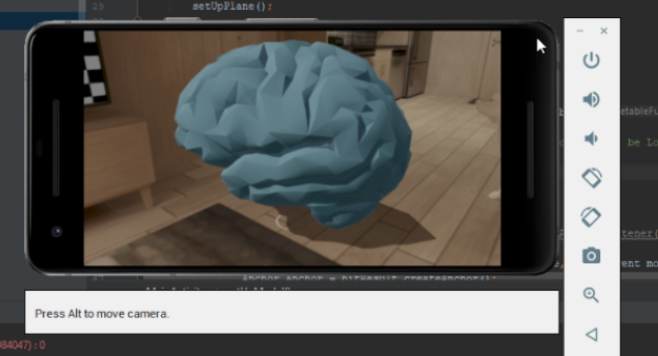
\includegraphics[width=.95\textwidth]{figuras/sceneform.png}
        \caption{Primeiro aplicativo AR para \textit{Android}}
        \label{fig:sceneform}
    \end{subfigure}
    \begin{subfigure}{0.45\textwidth}
        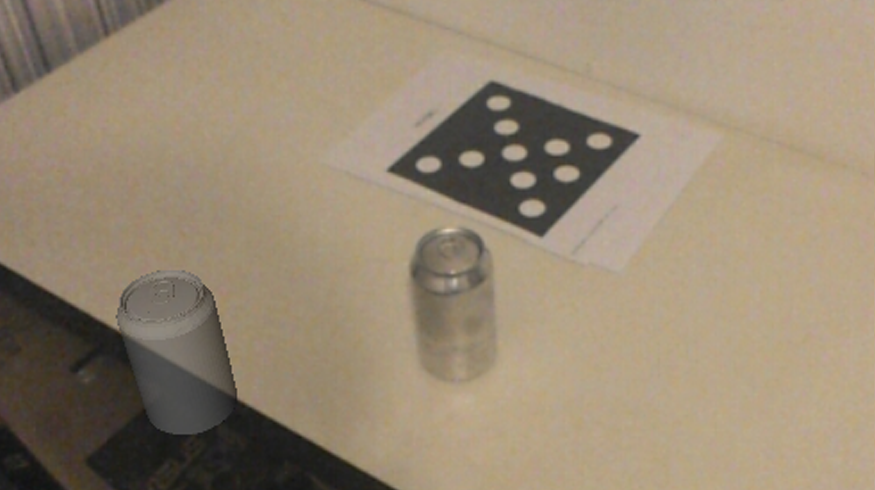
\includegraphics[width=.95\linewidth]{figuras/Latinha-errada.png}
        \caption{Tentativa de calibração do \textit{Moverio}}
        \label{fig:latinha}
    \end{subfigure}
    \begin{subfigure}{0.45\textwidth}
        \centering
        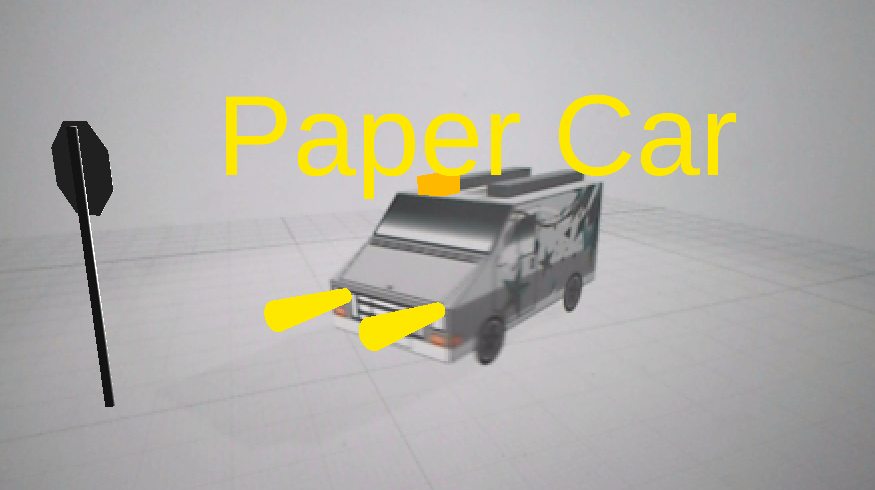
\includegraphics[width=.95\textwidth]{figuras/PaperCarAR.png}
        \caption{Aplicativo de exemplo fornecido pela \textit{EPSON}}
        \label{fig:papercar}
    \end{subfigure}
    \begin{subfigure}{0.45\textwidth}
        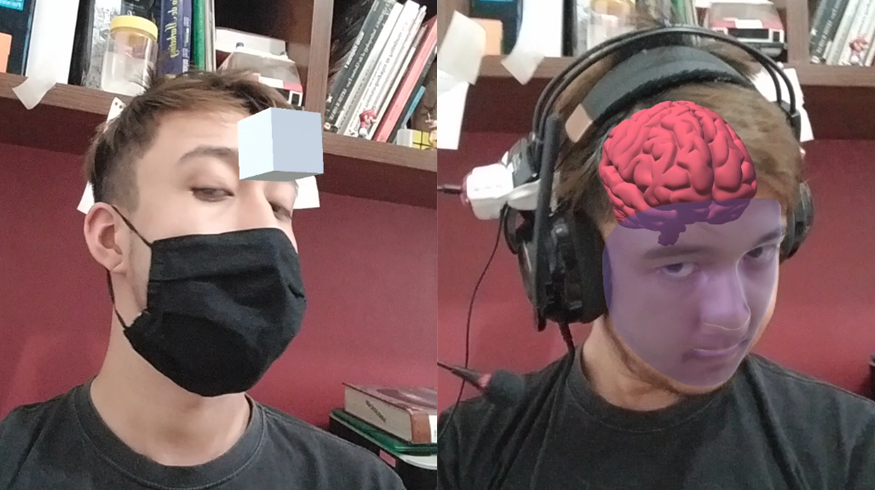
\includegraphics[width=.95\linewidth]{figuras/VCranium.png}
        \caption{Primeira versão do \textit{VCranium}}
        \label{fig:vcranium_alpha}
    \end{subfigure}
    \caption{Histórico de realizações da pesquisa até a primeira entrega parcial. Fonte: Autor.}
    \label{fig:historico}
\end{figure}


